\documentclass[aspectratio=169]{beamer}
\usetheme{Madrid}
\usecolortheme{default}
\usepackage[utf8]{inputenc}
\usepackage[T5]{fontenc}
\usepackage{graphicx}
\usepackage{hyperref}
\usepackage{booktabs}

\setbeamertemplate{caption}[numbered]
\renewcommand{\figurename}{Hình}
\renewcommand{\thefigure}{1.\arabic{figure}}

\title[Buổi 1: AI \& Nghề Kế toán]{Trí tuệ Nhân tạo cho Kế toán \\ \vspace{0.3cm} \Large Buổi 1: Những điều Kế toán viên cần biết về AI}
\author{Đại học Đông Á}
\date{\today}

\begin{document}

% SLIDE 1: TRANG BÌA
\begin{frame}
    \titlepage
\end{frame}

% SLIDE 2: NỘI DUNG CHƯƠNG TRÌNH
\begin{frame}{Nội dung Chương trình Buổi học (135 Phút)}
    \tableofcontents
\end{frame}

% SLIDE 3: MỤC TIÊU BÀI HỌC (LO)
\begin{frame}{Mục tiêu Bài học (Lesson Objectives - LO)}
    \begin{itemize}
        \item \textbf{LO 1.1 - Hiểu bản chất AI:} Nắm vững khái niệm Trí tuệ Nhân tạo trong tài chính, phân biệt rạch ròi giữa Trí tuệ con người, AI hẹp (ANI) và AI tổng quát (AGI).
        \item \textbf{LO 1.2 - Lịch sử \& Tiến hóa:} Hiểu hành trình phát triển của AI và 5 giai đoạn tiến hóa công nghệ của nghề Kế toán - Kiểm toán (từ bàn tính, Excel, ERP, Cloud đến AI).
        \item \textbf{LO 1.3 - Làm chủ Học máy \& Học sâu:} Giải thích được cơ chế hoạt động và ứng dụng tài chính của Học có giám sát, Học không giám sát, Học bán giám sát, Học tăng cường và Mạng nơ-ron Học sâu.
        \item \textbf{LO 1.4 - Tích hợp Hệ sinh thái Tự động hóa:} Phân tích sự kết hợp hiệu quả giữa Khai phá dữ liệu (Data Mining), NLP, RPA và API trong quy trình kế toán hiện đại.
        \item \textbf{LO 1.5 - Định hướng Công cụ:} Hiểu lý do vì sao Python là "ngôn ngữ chung" của Kế toán viên kỷ nguyên số và xây dựng lộ trình thăng tiến nghề nghiệp.
    \end{itemize}
\end{frame}

% ==============================================================================
% SECTION 1: KHÁI QUÁT VỀ AI & LỊCH SỬ CHUYỂN ĐỔI SỐ KẾ TOÁN
% ==============================================================================
\section{1. Khái quát về AI \& Lịch sử Chuyển đổi số Kế toán}

% SLIDE 4
\begin{frame}{1.1 Cuộc cách mạng AI trong nghề Kế toán}
    \begin{itemize}
        \item \textbf{Bối cảnh Kinh tế Số:} Dữ liệu tài chính không còn là những con số tĩnh trên sổ sách, mà đã trở thành "tài sản chiến lược" lớn nhất của doanh nghiệp.
        \item \textbf{Sự bùng nổ Dữ liệu Phi cấu trúc:} Hơn 80\% dữ liệu doanh nghiệp hiện nay là phi cấu trúc (hợp đồng kinh tế, hóa đơn scan, email, âm thanh, hình ảnh).
        \item \textbf{Thách thức của Kế toán truyền thống:} Các phương pháp thủ công và bảng tính đơn thuần không thể xử lý khối lượng dữ liệu khổng lồ này với tốc độ thời gian thực.
        \item \textbf{Yêu cầu Chuyển dịch Vai trò:} Kế toán viên đang bước qua giai đoạn từ "người ghi chép lịch sử" (Bookkeeper) sang "nhà phân tích và cố vấn chiến lược" (Strategic Business Advisor).
    \end{itemize}
\end{frame}

% SLIDE 5
\begin{frame}{1.2 Trí tuệ Nhân tạo (AI) là gì?}
    \begin{itemize}
        \item \textbf{Định nghĩa phổ quát:} Trí tuệ Nhân tạo (Artificial Intelligence) là khả năng của máy móc hoặc phần mềm thực hiện các tác vụ đòi hỏi nhận thức và suy luận tương tự con người.
        \item \textbf{Góc nhìn Tài chính - Kế toán:} AI không phải là "phép thuật thần kỳ", mà bản chất là sự kết hợp của toán học, thống kê nâng cao và năng lực xử lý máy tính trên tập dữ liệu lớn.
        \item \textbf{3 Trụ cột cốt lõi của AI hiện đại:}
        \begin{enumerate}
            \item \textbf{Dữ liệu (Data):} Hàng triệu chứng từ kế toán, sổ nhật ký, lịch sử giao dịch.
            \item \textbf{Thuật toán (Algorithms):} Mô hình toán học học hỏi từ dữ liệu để dự báo.
            \item \textbf{Sức mạnh Điện toán (Computing Power):} Điện toán đám mây và vi xử lý GPU/TPU tốc độ cao.
        \end{enumerate}
    \end{itemize}
\end{frame}

% SLIDE 6
\begin{frame}{1.3 Trí tuệ Con người vs. Trí tuệ Nhân tạo (P1)}
    \begin{columns}
        \column{0.5\textwidth}
        \textbf{Trí tuệ Con người (Human Intelligence):}
        \begin{itemize}
            \item Sở hữu \textbf{trực giác nghề nghiệp}, năng lực đánh giá đạo đức và sự thấu hiểu bối cảnh kinh doanh.
            \item Có khả năng giải quyết các tình huống "Thiên nga đen" (Black Swan) chưa từng có tiền lệ.
            \item \emph{Giới hạn:} Tốc độ tính toán chậm, dễ mệt mỏi, rủi ro sai sót khi lặp lại công việc cơ học.
        \end{itemize}
        
        \column{0.5\textwidth}
        \textbf{Trí tuệ Nhân tạo (AI):}
        \begin{itemize}
            \item Khả năng tính toán siêu tốc, xử lý hàng triệu hóa đơn trong vài giây với độ chính xác cao.
            \item Hoạt động liên tục 24/7/365, không mệt mỏi, không bị ảnh hưởng bởi tâm lý hay cảm xúc.
            \item \emph{Giới hạn:} Thiếu "ý thức" và "sự phán đoán đạo đức", phụ thuộc tuyệt đối vào chất lượng dữ liệu huấn luyện.
        \end{itemize}
    \end{columns}
\end{frame}

% SLIDE 7
\begin{frame}{1.4 Trí tuệ Con người vs. Trí tuệ Nhân tạo (P2)}
    \begin{table}
        \centering
        \small
        \begin{tabular}{p{4.2cm}p{4.8cm}p{4.8cm}}
            \toprule
            \textbf{Tiêu chí} & \textbf{AI Vượt trội} & \textbf{Con người Vượt trội} \\
            \midrule
            \textbf{Tác vụ lặp lại quy mô lớn} & Đối chiếu công nợ nghìn dòng, bóc tách OCR hóa đơn & Ít phù hợp (dễ mệt mỏi, sai sót) \\
            \textbf{Đánh giá \& Xét đoán} & Thống kê rủi ro theo mô hình & Xét đoán kế toán (Accounting Estimates) \\
            \textbf{Đạo đức \& Tuân thủ} & Tuân theo luật được lập trình & Thẩm định đạo đức IFRS/IFAC, giải trình \\
            \textbf{Tư vấn chiến lược} & Dự báo dòng tiền, chi phí & Thảo luận HĐQT, thương thảo hợp đồng \\
            \bottomrule
        \end{tabular}
    \end{table}
    \vspace{0.2cm}
    \textbf{Kết luận Sư phạm:} AI và Con người là mối quan hệ \textbf{bổ trợ (Augmentation)}, không phải đối đầu.
\end{frame}

% SLIDE 8
\begin{frame}{1.5 Lịch sử của Trí tuệ Nhân tạo (1950 - Nay)}
    \begin{itemize}
        \item \textbf{1950 - Phép thử Turing (Alan Turing):} Đặt nền móng triết học "Liệu máy móc có thể suy nghĩ?" qua bài kiểm tra khả năng giả lập giao tiếp con người.
        \item \textbf{1956 - Hội nghị Dartmouth:} Thuật ngữ "Artificial Intelligence" (Trí tuệ Nhân tạo) chính thức ra đời bởi John McCarthy và các nhà khoa học tiên phong.
        \item \textbf{1970 - 1980 - Kỷ nguyên Hệ chuyên gia (Expert Systems):} AI phát triển dựa trên luật suy diễn logic (Rule-based), ứng dụng đầu tiên trong chẩn đoán y khoa và thuế.
        \item \textbf{2010 - Hiện nay - Kỷ nguyên Học sâu \& Generative AI:} Sự bùng nổ của Mạng nơ-ron nhiều lớp (Deep Learning), Big Data và mô hình ngôn ngữ lớn (ChatGPT, Claude) làm thay đổi toàn diện ngành tài chính.
    \end{itemize}
\end{frame}

% SLIDE 9
\begin{frame}{1.6 Các "Mùa đông AI" \& Bài học Công nghệ}
    \begin{itemize}
        \item \textbf{Khái niệm "Mùa đông AI" (AI Winters):} Là những giai đoạn (1974-1980 và 1987-1993) khi sự ủng hộ và nguồn vốn nghiên cứu AI sụt giảm mạnh do không đạt được kỳ vọng thổi phồng.
        \item \textbf{Nguyên nhân trong quá khứ:}
        \begin{itemize}
            \item Phần cứng máy tính quá yếu, bộ nhớ hạn chế.
            \item Thiếu nguồn dữ liệu số hóa đủ lớn để huấn luyện mô hình.
            \item Thuật toán lý thuyết chưa giải quyết được bài toán phi tuyến tính phức tạp.
        \end{itemize}
        \item \textbf{Vì sao AI hiện đại không còn "Mùa đông"?:}
        \begin{itemize}
            \item Dữ liệu kế toán - tài chính đã số hóa 100\% (Cloud ERP, e-Invoice).
            \item Năng lực tính toán vi xử lý tăng cấp số nhân (GPU/TPU computing).
        \end{itemize}
    \end{itemize}
\end{frame}

% SLIDE 10
\begin{frame}{1.7 Lịch sử Kế toán ứng dụng Công nghệ (P1)}
    \begin{itemize}
        \item \textbf{Giai đoạn 1: Kỷ nguyên Thủ công \& Cơ học (Trước năm 1960)}
        \begin{itemize}
            \item Công cụ chủ đạo: Bàn tính (Abacus), Sổ sách kế toán giấy (Paper Ledgers).
            \item Đặc điểm: Tốc độ xử lý rất chậm, rủi ro sai sót tính toán thủ công cao, khó đối chiếu.
        \end{itemize}
        \item \textbf{Giai đoạn 2: Kỷ nguyên Máy tính Mainframe \& Bảng tính Điện tử (1960 - 1980)}
        \begin{itemize}
            \item Sự xuất hiện của phần mềm bảng tính ban đầu: VisiCalc (1979) và Lotus 1-2-3.
            \item Bước ngoặt lịch sử: \textbf{Microsoft Excel (1985)} ra đời, chuẩn hóa hoàn toàn công việc tính toán, bảng cân đối kế toán và tự động hóa công thức trên máy tính cá nhân.
        \end{itemize}
    \end{itemize}
\end{frame}

% SLIDE 11
\begin{frame}{1.8 Lịch sử Kế toán ứng dụng Công nghệ (P2)}
    \begin{itemize}
        \item \textbf{Giai đoạn 3: Kỷ nguyên Quản trị Nguồn lực Doanh nghiệp - ERP (1990 - 2000)}
        \begin{itemize}
            \item Các hệ thống ERP lớn (SAP, Oracle) kết nối liên thông dữ liệu giữa Phân hệ Bán hàng, Mua hàng, Kho hàng, Tài sản cố định và Sổ cái (General Ledger).
            \item Chấm dứt tình trạng "ốc đảo dữ liệu" (Data Silos) trong phòng Kế toán.
        \end{itemize}
        \item \textbf{Giai đoạn 4: Kỷ nguyên Điện toán Đám mây \& RPA (2000 - 2015)}
        \begin{itemize}
            \item Kế toán trên mây (Cloud Accounting: Xero, QuickBooks Online) cho phép truy cập tài chính mọi lúc mọi nơi.
            \item Tự động hóa Quy trình bằng Robot (RPA) bắt đầu thay thế việc copy-paste thủ công.
        \end{itemize}
    \end{itemize}
\end{frame}

% SLIDE 12
\begin{frame}{1.9 Kỷ nguyên Trí tuệ Nhân tạo trong Kế toán}
    \begin{itemize}
        \item \textbf{Giai đoạn 5: Kỷ nguyên AI \& Kiểm toán Liên tục (2015 - Hiện nay)}
        \begin{itemize}
            \item AI được tích hợp sâu vào cốt lõi các phần mềm kế toán và hệ thống quản trị tài chính doanh nghiệp.
        \end{itemize}
        \item \textbf{Sự chuyển dịch Mô hình Kiểm soát Tài chính:}
        \begin{itemize}
            \item \textbf{Trước đây:} Kiểm toán định kỳ (Periodic Auditing - Hậu kiểm sau tháng/quý/năm).
            \item \textbf{Hiện nay:} Kiểm toán liên tục (Continuous Auditing - Kiểm soát theo thời gian thực 24/7 nhờ thuật toán AI giám sát mọi bút toán).
        \end{itemize}
        \item \textbf{Báo cáo Tài chính Động:} Xuất báo cáo tài chính ngay tại thời điểm yêu cầu với năng lực dự báo dòng tiền tương lai có xác suất cao.
    \end{itemize}
\end{frame}

% SLIDE 13
\begin{frame}{1.10 Thực trạng Kế toán viên sử dụng AI}
    \begin{itemize}
        \item \textbf{Số liệu Thực tiễn từ Khảo sát Big4 \& AICPA:}
        \begin{itemize}
            \item Hơn 70\% doanh nghiệp kiểm toán lớn đã và đang triển khai các hệ thống AI trong kiểm tra hóa đơn và đánh giá rủi ro tín dụng.
            \item Việc áp dụng AI giúp tiết kiệm trung bình 40\% - 60\% thời gian xử lý hồ sơ chứng từ.
        \end{itemize}
        \item \textbf{3 Tác vụ AI đã trở thành Tiêu chuẩn ngành Kế toán:}
        \begin{enumerate}
            \item \textbf{Tự động xử lý Hóa đơn Điện tử (e-Invoice Processing):} Bóc tách dữ liệu không cần gõ phím.
            \item \textbf{Đối chiếu Ngân hàng Tự động (Automated Reconciliation):} Khớp lệnh nghìn giao dịch trong vài giây.
            \item \textbf{Phân tích Chi phí \& Phát hiện Ngoại lệ:} Cảnh báo các khoản chi sai định mức ngay lập tức.
        \end{enumerate}
    \end{itemize}
\end{frame}

% SLIDE 14
\begin{frame}{1.11 Thảo luận: AI có thay thế Kế toán viên?}
    \begin{itemize}
        \item \textbf{Câu hỏi Kinh điển:} "Liệu nghề Kế toán - Kiểm toán có biến mất trong tương lai vì sự phát triển của Trí tuệ Nhân tạo?"
        \item \textbf{Phân tích của Chuyên gia Tài chính:}
        \begin{itemize}
            \item AI chỉ thay thế các \textbf{tác vụ lặp đi lặp lại} (Bookkeeping, nhập liệu, đối chiếu cơ bản).
            \item AI KHÔNG THỂ thay thế tư duy xét đoán chuyên môn, trách nhiệm đạo đức giải trình và năng lực tư vấn chiến lược cho Giám đốc Tài chính (CFO).
        \end{itemize}
        \item \textbf{Khẩu hiệu Hành động của Môn học:}
        \begin{quote}
            "AI sẽ không thay thế Kế toán viên, nhưng Kế toán viên biết làm chủ AI chắc chắn sẽ thay thế Kế toán viên truyền thống!"
        \end{quote}
    \end{itemize}
\end{frame}

% ==============================================================================
% SECTION 2: HỆ SINH THÁI AI CỐT LÕI & HỌC MÁY TRONG TÀI CHÍNH
% ==============================================================================
\section{2. Hệ sinh thái AI Cốt lõi \& Học máy trong Tài chính}

% SLIDE 15
\begin{frame}{2.1 Phân loại Trí tuệ Nhân tạo: ANI vs. AGI}
    \begin{itemize}
        \item \textbf{2 Cấp độ Nhận thức và Độ rộng Tác vụ của AI:}
        \begin{enumerate}
            \item \textbf{Trí tuệ Nhân tạo Hẹp (ANI - Artificial Narrow Intelligence):} AI được lập trình và huấn luyện chuyên biệt để làm tốt MỘT tác vụ duy nhất.
            \item \textbf{Trí tuệ Nhân tạo Tổng quát (AGI - Artificial General Intelligence):} AI có khả năng nhận thức, tự suy luận và làm được mọi tác vụ trí tuệ như con người.
        \end{enumerate}
        \item \textbf{Trạng thái Ứng dụng Tài chính hiện tại:}
        \begin{itemize}
            \item 100\% các hệ thống AI đang áp dụng trong ngành Kế toán - Kiểm toán - Ngân hàng ngày nay đều thuộc phân lớp \textbf{ANI (AI Hẹp)}.
        \end{itemize}
    \end{itemize}
\end{frame}

% SLIDE 16
\begin{frame}{2.2 Trí tuệ Nhân tạo Hẹp (ANI) trong Kế toán}
    \begin{itemize}
        \item \textbf{Bản chất của ANI:} Siêu việt trong phạm vi nhỏ, nhưng hoàn toàn "mù tịt" nếu đưa ra khỏi lĩnh vực được huấn luyện.
        \item \emph{Ví dụ minh họa:} Mô hình AI đánh giá rủi ro tín dụng rất xuất sắc, nhưng không thể dùng mô hình đó để... đọc hiểu hợp đồng thuê tài sản.
        \item \textbf{3 Ví dụ ANI tiêu biểu trong ngành Kế toán:}
        \begin{enumerate}
            \item \textbf{AI-OCR:} Nhận diện ký tự và con số từ ảnh chụp hóa đơn GTGT.
            \item \textbf{Credit Risk Scoring:} Thuật toán chấm điểm tín dụng khách hàng dựa trên lịch sử thanh toán.
            \item \textbf{Chatbot Kế toán:} Trả lời tự động các quy định về Chuẩn mực IFRS 15 / IFRS 16.
        \end{enumerate}
    \end{itemize}
\end{frame}

% SLIDE 17
\begin{frame}{2.3 Trí tuệ Nhân tạo Tổng quát (AGI) \& Thách thức}
    \begin{itemize}
        \item \textbf{Tầm nhìn AGI trong tương lai:} Một "Kiểm toán viên máy móc" toàn năng có thể tự động đi tham quan nhà máy, nói chuyện với Giám đốc, phân tích sổ sách và tự đưa ra ý kiến kiểm toán.
        \item \textbf{Thách thức lớn về Đạo đức \& Kiểm soát (Value Alignment):}
        \begin{itemize}
            \item Làm thế nào để đảm bảo AGI tuân thủ tuyệt đối Đạo đức Nghề nghiệp Kế toán (IFAC / AICPA)?
            \item Ai sẽ là người chịu trách nhiệm pháp lý nếu AGI đưa ra quyết định sai sót gây thiệt hại hàng nghìn tỷ đồng?
            \item Kế toán viên cần tham gia vào quá trình thiết kế ranh giới đạo đức cho AI ngay từ bây giờ.
        \end{itemize}
    \end{itemize}
\end{frame}

% SLIDE 18
\begin{frame}{2.4 Lập luận máy (Machine Reasoning)}
    \begin{itemize}
        \item \textbf{Khái niệm Lập luận máy:} Là hệ thống AI biểu diễn tri thức dưới dạng các cấu trúc logic và sử dụng các thuật toán suy diễn để rút ra kết luận mới từ cơ sở dữ liệu hiện có.
        \item \textbf{2 Cơ chế Suy diễn cốt lõi trong Tài chính:}
        \begin{enumerate}
            \item \textbf{Liên kết Thuận (Forward Chaining):} Đi từ các sự kiện dữ liệu hiện có $\rightarrow$ Áp dụng các luật kế toán $\rightarrow$ Suy ra kết luận hạch toán cuối cùng.
            \item \textbf{Liên kết Ngược (Backward Chaining):} Đi từ một giả thuyết kiểm toán (Ví dụ: "Hóa đơn này vi phạm luật thuế") $\rightarrow$ Truy xuất ngược lại tìm dữ kiện chứng minh.
        \end{enumerate}
    \end{itemize}
\end{frame}

% SLIDE 19
\begin{frame}{2.5 Hệ chuyên gia (Expert Systems)}
    \begin{itemize}
        \item \textbf{Định nghĩa:} Hệ chuyên gia là một dạng AI sớm nhất và thành công nhất trong Kế toán, hoạt động bằng cách mô phỏng khả năng ra quyết định của một chuyên gia con người.
        \item \textbf{Cấu trúc 2 Thành phần Không thể tách rời:}
        \begin{enumerate}
            \item \textbf{Cơ sở Tri thức (Knowledge Base):} Tập hợp các chuẩn mực kế toán (VAS/IFRS), quy định Luật Thuế, chính sách tài chính được mã hóa dưới dạng \texttt{IF ... THEN ...}.
            \item \textbf{Động cơ Suy diễn (Inference Engine):} Thuật toán quét số liệu chứng từ thực tế và áp dụng luật từ Cơ sở Tri thức để đưa ra chỉ dẫn.
        \end{enumerate}
    \end{itemize}
\end{frame}

% SLIDE 20
\begin{frame}{2.6 Case Study: Hệ chuyên gia trong Tuân thủ Thuế}
    \begin{itemize}
        \item \textbf{Bài toán:} Kiểm tra tính hợp lệ của khoản chi phí được trừ thuế TNDN.
        \item \textbf{Chuỗi luật logic \texttt{IF - THEN} được mã hóa trong Hệ chuyên gia:}
        \begin{itemize}
            \item \texttt{IF} Hóa đơn có đầy đủ thông tin hợp lệ \texttt{AND} Không nằm trong danh sách doanh nghiệp bỏ trốn...
            \item \texttt{AND IF} Giá trị hóa đơn $\ge 20$ triệu VNĐ \texttt{THEN} Kiểm tra chứng từ thanh toán không dùng tiền mặt.
            \item \texttt{IF} Có ủy nhiệm chi hợp lệ \texttt{THEN} Phê duyệt khoản chi phí được trừ.
        \end{itemize}
        \item \textbf{Ưu điểm vượt trội:} Minh bạch tuyệt đối 100\%, có thể giải trình mọi bước suy diễn cho Đoàn thanh tra Thuế mà không bị "hộp đen" (Black Box).
    \end{itemize}
\end{frame}

% SLIDE 21
\begin{frame}{2.7 Học máy (Machine Learning - ML)}
    \begin{itemize}
        \item \textbf{Định nghĩa của Arthur Samuel (1959):} Học máy là lĩnh vực của Trí tuệ Nhân tạo cung cấp cho máy tính khả năng tự học hỏi từ dữ liệu mà không cần phải được lập trình tường minh từng quy tắc.
        \item \textbf{Sự khác biệt mang tính Cách mạng:}
        \begin{itemize}
            \item \textbf{Lập trình Kế toán Truyền thống:} Con người nạp \texttt{[Dữ liệu Sổ sách]} + \texttt{[Quy tắc/Luật Hạch toán]} vào máy $\rightarrow$ Máy tính ra \texttt{[Kết quả Báo cáo]}.
            \item \textbf{Học máy (Machine Learning):} Con người nạp \texttt{[Dữ liệu Sổ sách]} + \texttt{[Kết quả/Nhãn Thực tế]} vào máy $\rightarrow$ Máy tự học và tạo ra \texttt{[Quy luật Thuật toán]}.
        \end{itemize}
    \end{itemize}
\end{frame}

% SLIDE 22
\begin{frame}{2.8 Sơ đồ Mối quan hệ: AI - ML - DL}
    \begin{columns}
        \column{0.55\textwidth}
        \begin{itemize}
            \item \textbf{Trí tuệ Nhân tạo (AI):} Lĩnh vực khoa học rộng lớn bao hàm mọi kỹ thuật giúp máy thông minh.
            \item \textbf{Học máy (Machine Learning - ML):} Tập con của AI, sử dụng thuật toán thống kê tự học quy luật từ dữ liệu kế toán lịch sử.
            \item \textbf{Học sâu (Deep Learning - DL):} Tập con của ML, sử dụng Mạng nơ-ron đa tầng xử lý dữ liệu phi cấu trúc.
        \end{itemize}
        
        \column{0.45\textwidth}
        \begin{figure}
            \centering
            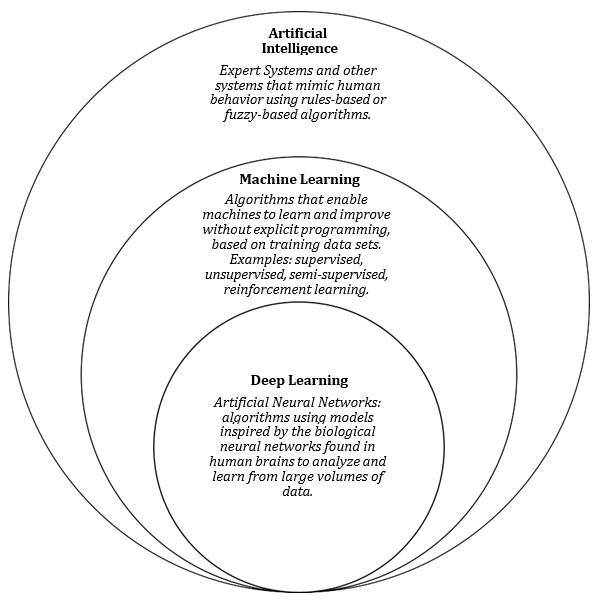
\includegraphics[width=\textwidth,height=0.75\textheight,keepaspectratio]{../../Figures/Buoi_01/Figure 1.1 Relationship between AI, ML, and DL..PNG}
            \caption{Mối quan hệ giữa AI, ML và DL}
        \end{figure}
    \end{columns}
\end{frame}

% SLIDE 23
\begin{frame}{2.9 Phân tích Biểu đồ Figure 1.1}
    \begin{itemize}
        \item \textbf{Diễn giải Sơ đồ Euler dưới góc độ Kế toán - Kiểm toán:}
        \begin{enumerate}
            \item \textbf{Trí tuệ Nhân tạo (AI - Vòng lớn ngoài cùng):} Là toàn bộ lĩnh vực khoa học rộng lớn bao gồm mọi kỹ thuật giúp máy thông minh (bao gồm Hệ chuyên gia, RPA, Học máy).
            \item \textbf{Học máy (ML - Vòng giữa):} Là một tập con thuộc AI, sử dụng các thuật toán thống kê tự học quy luật từ dữ liệu kế toán lịch sử.
            \item \textbf{Học sâu (Deep Learning - DL - Vòng trong cùng):} Là một tập con thuộc ML, sử dụng Mạng nơ-ron nhân tạo đa tầng để xử lý dữ liệu phức tạp phi cấu trúc.
        \end{enumerate}
        \item \emph{Quy tắc vàng: "Mọi Học sâu đều là Học máy, và mọi Học máy đều là Trí tuệ nhân tạo, nhưng điều ngược lại thì không đúng!"}
    \end{itemize}
\end{frame}

% SLIDE 24
\begin{frame}{2.10 Học có giám sát (Supervised Learning - P1)}
    \begin{itemize}
        \item \textbf{Cơ chế hoạt động:} Mô hình được huấn luyện trên tập dữ liệu đã có nhãn đích rõ ràng (Labeled Data). Kế toán viên đóng vai trò "người thầy" chỉ cho máy biết câu trả lời đúng.
        \item \textbf{2 Bài toán cốt lõi của Học có giám sát:}
        \begin{enumerate}
            \item \textbf{Bài toán Phân lớp (Classification):} Dự báo nhãn rời rạc theo từng nhóm (Ví dụ: `Gian lận` / `Hợp lệ` ; `Vỡ nợ` / `An toàn`).
            \item \textbf{Bài toán Hồi quy (Regression):} Dự báo một giá trị số liên tục (Ví dụ: Dự báo Doanh thu quý tới là `150.5 Tỷ VNĐ`).
        \end{enumerate}
    \end{itemize}
\end{frame}

% SLIDE 25
\begin{frame}{2.11 Học có giám sát trong Kế toán (P2)}
    \begin{itemize}
        \item \textbf{Ứng dụng 1: Phát hiện Gian lận Hóa đơn (Fraud Detection)}
        \begin{itemize}
            \item Huấn luyện mô hình trên 50,000 hóa đơn lịch sử (đã được Kiểm toán viên gán nhãn: `0 = Hợp lệ`, `1 = Gian lận`).
            \item Khi hóa đơn mới xuất hiện, mô hình tự động chấm điểm xác suất gian lận để cảnh báo phòng Kế toán.
        \end{itemize}
        \item \textbf{Ứng dụng 2: Chấm điểm Tín dụng Khách hàng (Credit Scoring)}
        \begin{itemize}
            \item Dựa trên các chỉ số tài chính (hệ số thanh toán, lịch sử trả nợ), phân loại khách hàng có nợ phải thu vào nhóm `Rủi ro cao`, `Rủi ro trung bình`, hay `Rủi ro thấp`.
        \end{itemize}
    \end{itemize}
\end{frame}

% SLIDE 26
\begin{frame}{2.12 Học không giám sát (Unsupervised Learning - P1)}
    \begin{itemize}
        \item \textbf{Cơ chế hoạt động:} Thuật toán làm việc với tập dữ liệu hoàn toàn KHÔNG CÓ NHÃN (Unlabeled Data). Máy tính tự tìm kiếm mô hình, cấu trúc và sự tương đồng ngầm trong dữ liệu.
        \item \textbf{2 Kỹ thuật chủ đạo trong Phân tích Tài chính:}
        \begin{enumerate}
            \item \textbf{Phân cụm (Clustering - K-Means, DBSCAN):} Gom nhóm các giao dịch hoặc đối tượng tài chính có hành vi tương tự nhau.
            \item \textbf{Giảm số chiều (Dimensionality Reduction - PCA):} Đơn giản hóa hàng trăm biến số tài chính xuống còn vài nhân tố chính mà không mất thông tin.
        \end{enumerate}
    \end{itemize}
\end{frame}

% SLIDE 27
\begin{frame}{2.13 Học không giám sát trong Kiểm toán (P2)}
    \begin{itemize}
        \item \textbf{Ứng dụng Đột phá: Phát hiện Giao dịch Bất thường (Anomaly Detection)}
        \begin{itemize}
            \item Kiểm toán viên không thể biết trước hình thái của mọi hành vi gian lận mới.
            \item Thuật toán Học không giám sát tự động phân cụm hàng triệu bút toán trong Sổ Nhật ký chung (General Ledger) và lập tức khoanh vùng các giao dịch "lạc loài" (Outliers):
            \item \textbf{Ví dụ 1:} Bút toán chuyển tiền phát sinh lúc 3:00 sáng ngày Chủ Nhật.
            \item \textbf{Ví dụ 2:} Hàng loạt giao dịch mua thiết bị có giá trị \texttt{19,990,000 VNĐ} (né ngưỡng phê duyệt 20 triệu).
        \end{itemize}
    \end{itemize}
\end{frame}

% SLIDE 28
\begin{frame}{2.14 Học bán giám sát (Semi-supervised Learning)}
    \begin{itemize}
        \item \textbf{Bài toán Thực tế của Kế toán viên:}
        \begin{itemize}
            \item Doanh nghiệp có 1,000,000 hóa đơn mỗi năm, nhưng Kế toán viên chỉ có đủ thời gian kiểm tra chi tiết và gán nhãn cho 50,000 hóa đơn (5\% dữ liệu).
            \item 95\% dữ liệu còn lại là dữ liệu không nhãn.
        \end{itemize}
        \item \textbf{Giải pháp Học bán giám sát:}
        \begin{itemize}
            \item Mô hình học từ 5\% dữ liệu có nhãn để hiểu quy luật, sau đó lan truyền nhận thức sang 95\% dữ liệu không nhãn.
            \item Tiết kiệm đến 80\% chi phí và công sức kiểm toán thủ công nhưng vẫn đạt độ chính xác rất cao.
        \end{itemize}
    \end{itemize}
\end{frame}

% SLIDE 29
\begin{frame}{2.15 Học tăng cường (Reinforcement Learning - P1)}
    \begin{itemize}
        \item \textbf{Cơ chế hoạt động:} Tác nhân AI (Agent) tự học thông qua quá trình \textbf{Thử \& Sai (Trial and Error)} trong một môi trường động tương tự như chơi một trò chơi tài chính.
        \item \textbf{Hệ thống Phần thưởng \& Hình phạt (Reward System):}
        \begin{itemize}
            \item Nếu quyết định tài chính đem lại lợi nhuận/giảm rủi ro $\rightarrow$ Máy được nhận phần thưởng (+).
            \item Nếu quyết định dẫn đến lỗ hoặc vi phạm ràng buộc $\rightarrow$ Máy bị hình phạt (-).
            \item Thuật toán tự động tối ưu hóa chiến lược hành động để đạt tổng phần thưởng kỳ vọng lớn nhất sau hàng triệu kịch bản mô phỏng.
        \end{itemize}
    \end{itemize}
\end{frame}

% SLIDE 30
\begin{frame}{2.16 Học tăng cường trong Tài chính (P2)}
    \begin{itemize}
        \item \textbf{Ứng dụng 1 - Quản trị Dòng tiền Động (Dynamic Cash Management):}
        \begin{itemize}
            \item Tác nhân RL tự động cân đối lượng tiền mặt giữ lại tại quỹ và số tiền đem gửi tiết kiệm ngắn hạn dựa trên biến động lãi suất hằng ngày.
        \end{itemize}
        \item \textbf{Ứng dụng 2 - Chiến lược Định giá Động (Dynamic Pricing):}
        \begin{itemize}
            \item Tự động điều chỉnh giá bán sản phẩm theo thời gian thực dựa trên nhu cầu thị trường, lượng hàng tồn kho và giá đối thủ, nhằm tối đa hóa biên lợi nhuận gộp.
        \end{itemize}
    \end{itemize}
\end{frame}

% SLIDE 31
\begin{frame}{2.17 Học sâu (Deep Learning - DL)}
    \begin{itemize}
        \item \textbf{Cấu trúc Mạng Thần kinh Nhân tạo Đa tầng (Deep Neural Networks - DNN):}
        \begin{itemize}
            \item Gồm các lớp Nơ-ron đầu vào (Input Layer), nhiều lớp ẩn (Hidden Layers) và lớp đầu ra (Output Layer).
        \end{itemize}
        \item \textbf{Năng lực vượt trội với Dữ liệu Phi cấu trúc:}
        \begin{itemize}
            \item Không cần con người làm bước "trích xuất đặc trưng thủ công" (Feature Engineering).
            \item DL tự động nhận biết đường nét, chữ viết, ký hiệu trên hóa đơn chụp bị mờ, nghiêng, hoặc file ghi âm cuộc họp hội đồng quản trị.
        \end{itemize}
    \end{itemize}
\end{frame}

% ==============================================================================
% SECTION 3: NLP, KHAI PHÁ DỮ LIỆU, RPA & API CHO KẾ TOÁN
% ==============================================================================
\section{3. NLP, Khai phá Dữ liệu, RPA \& API cho Kế toán}

% SLIDE 32
\begin{frame}{3.1 Ứng dụng DL: Tự động hóa Chứng từ (OCR + AI)}
    \begin{itemize}
        \item \textbf{Bước tiến từ OCR Truyền thống sang IDP (Intelligent Document Processing):}
        \begin{itemize}
            \item OCR truyền thống chỉ chụp ảnh và đoán ký tự, dễ sai khi hóa đơn thay đổi biểu mẫu.
            \item IDP ứng dụng Học sâu (Deep Learning) để \textbf{hiểu ngữ cảnh}: Biết đâu là Tên người bán, đâu là Mã số thuế, đâu là Tổng tiền VAT dù biểu mẫu mới gặp lần đầu.
        \end{itemize}
        \item \textbf{Quy trình Hạch toán Tự động hoàn toàn:}
        \begin{itemize}
            \item \texttt{[Ảnh Hóa đơn PDF]} $\rightarrow$ \texttt{[DL-OCR trích xuất]} $\rightarrow$ \texttt{[ML đối chiếu Đơn hàng PO]} $\rightarrow$ \texttt{[Tự động tạo Bút toán trên Sổ cái]}.
        \end{itemize}
    \end{itemize}
\end{frame}

% SLIDE 33
\begin{frame}{3.2 Xử lý Ngôn ngữ Tự nhiên (NLP - P1)}
    \begin{itemize}
        \item \textbf{Khái niệm NLP (Natural Language Processing):}
        \begin{itemize}
            \item Là nhánh của AI chuyên giúp máy tính hiểu, diễn giải và sinh ra ngôn ngữ của con người dưới dạng văn bản hoặc giọng nói.
        \end{itemize}
        \item \textbf{2 Phân hệ Cốt lõi của NLP:}
        \begin{enumerate}
            \item \textbf{Hiểu Ngôn ngữ Tự nhiên (NLU - Natural Language Understanding):} Phân tích ý nghĩa, ngữ pháp và cảm xúc của bài viết kinh tế.
            \item \textbf{Sinh Ngôn ngữ Tự nhiên (NLG - Natural Language Generation):} Tự động soạn thảo văn bản giải trình tài chính mạch lạc như con người viết.
        \end{enumerate}
    \end{itemize}
\end{frame}

% SLIDE 34
\begin{frame}{3.3 NLP trong Kế toán - Kiểm toán (P2)}
    \begin{itemize}
        \item \textbf{Ứng dụng 1: Phân tích Hợp đồng Kinh tế (Contract Analysis)}
        \begin{itemize}
            \item NLP tự động đọc hợp đồng thuê tài sản dài 50 trang, trích xuất chính xác các điều khoản về thời hạn, lãi suất, quyền mua lại để hạch toán đúng Chuẩn mực IFRS 16.
        \end{itemize}
        \item \textbf{Ứng dụng 2: Trợ lý Ảo cho Giám đốc Tài chính (CFO Chatbot)}
        \begin{itemize}
            \item CFO hỏi: "Doanh thu dòng sản phẩm A tháng này giảm vì sao?" $\rightarrow$ NLP phân tích dữ liệu ERP và trả lời ngay lý do chi tiết bằng ngôn ngữ tự nhiên.
        \end{itemize}
    \end{itemize}
\end{frame}

% SLIDE 35
\begin{frame}{3.4 Khai phá Dữ liệu (Data Mining)}
    \begin{itemize}
        \item \textbf{Định nghĩa Khai phá Dữ liệu:}
        \begin{itemize}
            \item Là quá trình phân tích sâu các kho dữ liệu lớn (Data Warehouse) bằng công cụ toán học và AI để tìm ra các mẫu hình (Patterns), xu hướng ẩn và mối tương quan kinh tế.
        \end{itemize}
        \item \textbf{Khác biệt với Thống kê Kế toán truyền thống:}
        \begin{itemize}
            \item Thống kê truyền thống: "Đúng hay sai giả thuyết có sẵn?"
            \item Khai phá dữ liệu: "Hãy khám phá xem dữ liệu đang ẩn chứa quy luật vàng nào mà Kế toán viên chưa từng nghĩ tới!"
        \end{itemize}
    \end{itemize}
\end{frame}

% SLIDE 36
\begin{frame}{3.5 Sơ đồ: Big Data Mining và AI}
    \begin{columns}
        \column{0.55\textwidth}
        \begin{itemize}
            \item \textbf{Dữ liệu lớn (Big Data):} Mỏ quặng khổng lồ chứa hàng tỷ giao dịch bán hàng, nhật ký hệ thống, dữ liệu thị trường.
            \item \textbf{Khai phá Dữ liệu (Data Mining):} Kỹ thuật sàng lọc quặng, trích xuất ra các mô hình (Models) có giá trị kinh tế.
            \item \textbf{Trí tuệ Nhân tạo (AI):} Sử dụng các mô hình khai phá được để ra quyết định và tự động hóa tác vụ tài chính.
        \end{itemize}
        
        \column{0.45\textwidth}
        \begin{figure}
            \centering
            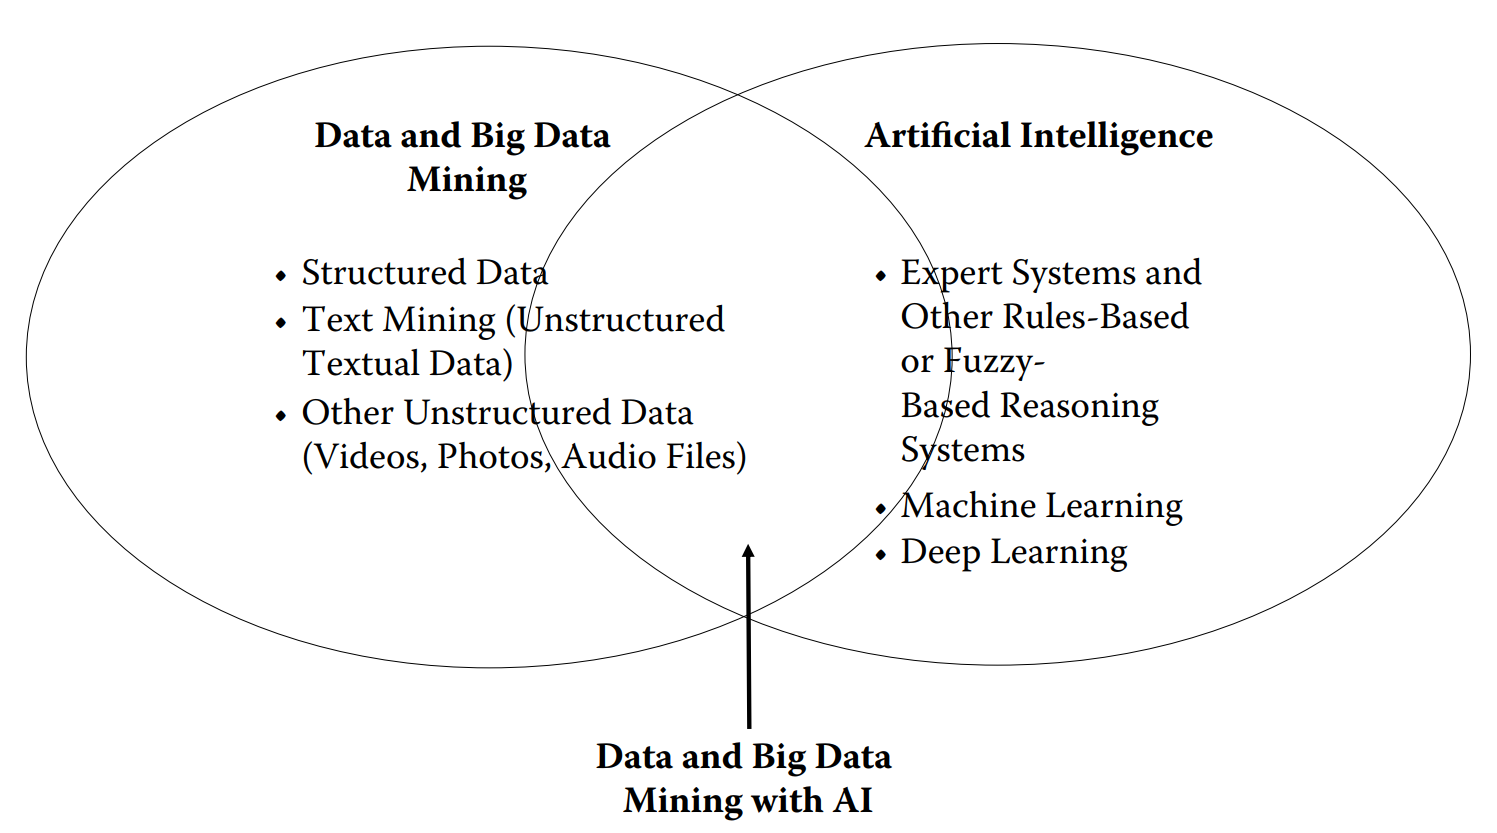
\includegraphics[width=\textwidth,height=0.75\textheight,keepaspectratio]{../../Figures/Buoi_01/Figure 1.2 Relationship between (big) data mining and AI..PNG}
            \caption{Mối quan hệ giữa Data Mining và AI}
        \end{figure}
    \end{columns}
\end{frame}

% SLIDE 37
\begin{frame}{3.6 Phân tích Biểu đồ Figure 1.2}
    \begin{itemize}
        \item \textbf{Diễn giải Biểu đồ Figure 1.2 trong Kế toán Quản trị:}
        \begin{enumerate}
            \item \textbf{Dữ liệu lớn (Big Data):} Là mỏ quặng khổng lồ chứa hàng tỷ bản ghi giao dịch bán hàng, nhật ký hệ thống, dữ liệu thị trường.
            \item \textbf{Khai phá Dữ liệu (Data Mining):} Là công nghệ sàng lọc quặng, trích xuất ra các mô hình (Models) có giá trị kinh tế cao.
            \item \textbf{Trí tuệ Nhân tạo (AI):} Sử dụng các mô hình khai phá được để ra quyết định và tự động hóa tác vụ tài chính thời gian thực.
        \end{enumerate}
    \end{itemize}
\end{frame}

% SLIDE 38
\begin{frame}{3.7 Khai phá Văn bản (Text Mining)}
    \begin{itemize}
        \item \textbf{Khái niệm Khai phá Văn bản:}
        \begin{itemize}
            \item Là kỹ thuật chuyên sâu của Data Mining nhằm trích xuất thông tin có giá trị từ dữ liệu văn bản phi cấu trúc (Text-based Data).
        \end{itemize}
        \item \textbf{Ứng dụng trong Kế toán - Kiểm toán \& Đầu tư:}
        \begin{enumerate}
            \item \textbf{Phân tích Cảm xúc (Sentiment Analysis):} Đo lường tông giọng lạc quan hay bi quan của HĐQT trong Báo cáo Thường niên (Annual Reports) để dự báo giá cổ phiếu.
            \item \textbf{Rà soát Pháp lý:} Quét tự động biên bản họp hội đồng thành viên để tìm cảnh báo rủi ro gian lận, kiện tụng tiềm ẩn.
        \end{enumerate}
    \end{itemize}
\end{frame}

% SLIDE 39
\begin{frame}{3.8 Tự động hóa Quy trình bằng Robot (RPA)}
    \begin{itemize}
        \item \textbf{Khái niệm RPA (Robotic Process Automation):}
        \begin{itemize}
            \item Sử dụng "Robot phần mềm" để bắt chước các thao tác máy tính của con người trên giao diện người dùng (GUI) nhằm thực hiện các tác vụ lặp lại theo quy tắc.
        \end{itemize}
        \item \textbf{Hành vi tiêu biểu của Robot RPA trong Kế toán:}
        \begin{itemize}
            \item Tự động đăng nhập vào Cổng dịch vụ Ngân hàng $\rightarrow$ Tải Sổ phụ ngân hàng hằng ngày $\rightarrow$ Mở phần mềm Kế toán $\rightarrow$ Nhập liệu đối chiếu số dư mà không cần con người bấm chuột.
        \end{itemize}
    \end{itemize}
\end{frame}

% SLIDE 40
\begin{frame}{3.9 Tiến hóa: Từ RPA truyền thống đến AI-RPA}
    \begin{itemize}
        \item \textbf{RPA Truyền thống (Blind Robot - Robot mù):}
        \begin{itemize}
            \item Hoạt động thuần túy theo quy tắc cố định (Rule-based: Cứ click vào tọa độ X, Y).
            \item Gặp một hóa đơn đổi mẫu mã hay mạng internet lag nhẹ là Robot... treo hệ thống và báo lỗi.
        \end{itemize}
        \item \textbf{AI-RPA (Intelligent Automation - Tự động hóa thông minh):}
        \begin{itemize}
            \item Sự dung hợp giữa \textbf{RPA + AI (OCR + Machine Learning + NLP)}.
            \item Robot không chỉ "click và paste", mà có năng lực HIỂU chứng từ, tự xử lý ngoại lệ và tự học biểu mẫu mới.
        \end{itemize}
    \end{itemize}
\end{frame}

% SLIDE 41
\begin{frame}{3.10 Case Study RPA + AI trong Kế toán}
    \begin{itemize}
        \item \textbf{Quy trình Tự động hóa Kế toán Thanh toán (Accounts Payable - AP):}
        \item \textbf{Các bước tự động liên hoàn không chậm trễ:}
        \begin{enumerate}
            \item \textbf{Bước 1 (RPA):} Đúng 8:00 sáng, Robot tự tải 500 file hóa đơn PDF từ hòm thư điện tử của nhà cung cấp.
            \item \textbf{Bước 2 (AI-IDP):} Học sâu đọc và bóc tách dữ liệu chi tiết từng dòng hóa đơn.
            \item \textbf{Bước 3 (ML):} Thuật toán đối chiếu tự động 3 bên (3-Way Matching: Hóa đơn == Đơn mua hàng PO == Phiếu nhập kho GRN).
            \item \textbf{Bước 4 (RPA):} Tự động lập lệnh chi trên hệ thống Ngân hàng cho các chứng từ khớp 100\%; chỉ báo cáo Kế toán viên các trường hợp lệch giá.
        \end{enumerate}
    \end{itemize}
\end{frame}

% SLIDE 42
\begin{frame}{3.11 Giao diện Lập trình Ứng dụng (API) \& AI (P1)}
    \begin{itemize}
        \item \textbf{Khái niệm API (Application Programming Interface):}
        \begin{itemize}
            \item Là bộ quy ước giao tiếp chuẩn hóa cho phép các phần mềm và hệ thống máy tính khác nhau "trò chuyện" và chia sẻ dữ liệu trực tiếp với nhau.
        \end{itemize}
        \item \textbf{Chấm dứt Kỷ nguyên Nhập liệu Thủ công:}
        \begin{itemize}
            \item Kế toán viên không còn phải xuất file Excel từ hệ thống bán hàng (POS) rồi hì hục import/nhập lại vào phần mềm Kế toán. API đồng bộ dữ liệu ngay lập tức từng giây.
        \end{itemize}
    \end{itemize}
\end{frame}

% SLIDE 43
\begin{frame}{3.12 Tích hợp API và AI trong Kế toán (P2)}
    \begin{itemize}
        \item \textbf{Hệ sinh thái Kế toán Mở (Open Accounting APIs):}
        \begin{enumerate}
            \item \textbf{Gọi API sang Mô hình AI:} Phần mềm kế toán khi tạo đơn bán hàng sẽ tự động gọi API sang mô hình AI trên đám mây để chấm điểm hạn mức tín dụng khách hàng trong 0.1 giây.
            \item \textbf{API Thuế Điện tử:} Tự động truyền thẳng dữ liệu hóa đơn điện tử và Báo cáo quyết toán thuế lên Cổng thông tin Tổng cục Thuế với chữ ký số được mã hóa bảo mật.
        \end{enumerate}
    \end{itemize}
\end{frame}

% ==============================================================================
% SECTION 4: CÔNG CỤ LẬP TRÌNH (PYTHON/SQL) & LỘ TRÌNH KỸ NĂNG
% ==============================================================================
\section{4. Công cụ Lập trình (Python/SQL) \& Lộ trình Kỹ năng}

% SLIDE 44
\begin{frame}{4.1 Ngôn ngữ Lập trình tốt nhất cho Kế toán viên}
    \begin{itemize}
        \item \textbf{3 "Vũ khí Công nghệ" vàng cho Kế toán viên hiện đại:}
        \begin{enumerate}
            \item \textbf{Python:} Ngôn ngữ số 1 toàn cầu cho AI, Học máy, Xử lý dữ liệu tài chính lớn và viết kịch bản tự động hóa Kế toán.
            \item \textbf{R:} Ngôn ngữ cực mạnh trong Thống kê toán học chuyên sâu, kiểm định mô hình rủi ro và Kiểm toán phân tích.
            \item \textbf{SQL (Structured Query Language):} Ngôn ngữ truy vấn cơ sở dữ liệu nền tảng, giúp Kế toán viên trực tiếp lấy số liệu từ kho dữ liệu ERP mà không cần nhờ IT.
        \end{enumerate}
    \end{itemize}
\end{frame}

% SLIDE 45
\begin{frame}{4.2 Vì sao Kế toán viên hiện đại chọn Python?}
    \begin{itemize}
        \item \textbf{4 Lý do Chiến lược khiến Python là "Ngôn ngữ chung":}
        \begin{enumerate}
            \item \textbf{Cú pháp cực kỳ trực quan:} Dễ đọc, dễ viết như tiếng Anh tự nhiên, học nhanh chóng ngay cả với sinh viên khối kinh tế - kế toán.
            \item \textbf{Thư viện Kế toán/Tài chính vô địch:} \texttt{pandas} (bảng tính lớn), \texttt{scikit-learn} (học máy), \texttt{matplotlib/seaborn} (trực quan hóa).
            \item \textbf{Tích hợp sâu với Excel \& ERP:} Tự động hóa xử lý hàng trăm file Excel trong 5 giây.
            \item \textbf{Cộng đồng toàn cầu:} Hàng triệu kế toán viên lập trình hỗ trợ giải đáp mã nguồn mở.
        \end{enumerate}
    \end{itemize}
\end{frame}

% SLIDE 46
\begin{frame}{4.3 Lộ trình Nâng cấp Năng lực (Upskilling Roadmap)}
    \begin{itemize}
        \item \textbf{4 Bước Phát triển Năng lực AI cho Kế toán viên:}
        \begin{enumerate}
            \item \textbf{Bước 1 - Năng lực Dữ liệu (Data Literacy):} Rèn luyện tư duy số, hiểu cấu trúc bảng biểu và nguyên tắc bảo mật dữ liệu tài chính.
            \item \textbf{Bước 2 - Làm chủ Công cụ Quản trị:} Thành thạo Excel nâng cao (Power Query, Power Pivot) và câu lệnh SQL cơ bản để truy xuất dữ liệu ERP.
            \item \textbf{Bước 3 - Học lập trình Python Kế toán:} Viết script tự động hóa công việc thường nhật và phân tích dữ liệu thăm dò (EDA).
            \item \textbf{Bước 4 - Triển khai AI \& RPA:} Tích hợp các mô hình Học máy, NLP và Trợ lý AI vào quy trình nghiệp vụ thực tế của doanh nghiệp.
        \end{enumerate}
    \end{itemize}
\end{frame}

% SLIDE 47
\begin{frame}{4.4 Bài tập Ôn tập Tình huống Buổi 1}
    \begin{itemize}
        \item \textbf{Đề bài Thực hành - Hãy chọn Công nghệ AI đúng:}
        \item \emph{Hãy xác định công nghệ phù hợp nhất (\textbf{Supervised ML, Unsupervised ML, NLP, RPA, hay Expert System}) cho 4 bài toán sau:}
        \begin{enumerate}
            \item \textbf{Tình huống 1:} Tự động mở website ngân hàng, tải sổ phụ, copy số dư vào phần mềm kế toán vào 7:00 sáng mỗi ngày.
            \item \textbf{Tình huống 2:} Phân tích 20,000 khách hàng để gom thành 4 nhóm có hành vi mua sắm và thanh toán giống nhau mà không biết trước nhóm nào.
            \item \textbf{Tình huống 3:} Xây dựng hệ thống kiểm tra tự động xem một khoản vay ngân hàng có tuân thủ đúng định mức tỷ lệ nợ trên vốn theo Luật Thuế hay không.
            \item \textbf{Tình huống 4:} Đọc file hợp đồng kinh tế PDF và cảnh báo các điều khoản vi phạm chuẩn mực kế toán IFRS 15.
        \end{enumerate}
    \end{itemize}
\end{frame}

% SLIDE 48
\begin{frame}{4.5 Tổng kết Buổi 1 \& Lời dặn dò Buổi 2}
    \begin{itemize}
        \item \textbf{5 Điểm Ghi nhớ Cốt lõi của Buổi 1:}
        \begin{enumerate}
            \item AI không thay thế Kế toán viên; AI mở rộng năng lực và tầm ảnh hưởng của Kế toán viên.
            \item Phân biệt rõ Trí tuệ con người vs. AI Hẹp (ANI) vs. AI Tổng quát (AGI).
            \item Học máy (Supervised, Unsupervised, RL) \& Học sâu là động cơ chuyển đổi số tài chính.
            \item Data Mining, NLP, RPA và API kết hợp tạo nên hệ sinh thái tự động hóa trọn vẹn.
            \item Python và SQL là chìa khóa thăng tiến trong nghề Kế toán kỷ nguyên số.
        \end{enumerate}
        \item \textbf{Dặn dò chuẩn bị cho Buổi 2:}
        \begin{itemize}
            \item Đọc trước tài liệu PDF trong thư mục \texttt{textbook} cho Buổi 2: \textbf{"AI and Finance, Big Data \& Blockchain"}.
            \item Chuẩn bị câu hỏi thảo luận về cách Big Data và Blockchain thay đổi chứng từ kế toán.
        \end{itemize}
    \end{itemize}
\end{frame}

\end{document}
